





\section{Can Fine-Tuning Close the \textbf{DENSEWORLD} Gap?}
\label{sec:vjepa_adaptation_baselines}

Before introducing FactorJEPA, we ask whether conventional adaptation can recover the predictive structure required by DENSEWORLD without reorganizing the JEPA predictor. We evaluate three complementary strategies: \textbf{LoRA}~\cite{hu2022lora}, \textbf{DoRA}~\cite{liu2024dora}, and \textbf{Auto-RGN}~\cite{lee2023surgical}. All use the same raw clips, optimization steps, optimizer, masking policy, and evaluation protocol; only the parameter-update mechanism changes.

Let $x$ denote a video clip; $M_c$ and $M_t$ the context and target masks; $f_\theta$ the online encoder; $\bar f_{\bar\theta}$ the momentum target encoder; and $g_\phi$ the predictor. All baselines retain the executed V-JEPA objective:
\[
\mathcal{L}_{\mathrm{JEPA}}
=
\mathbb{E}_{x}
\left[
\left\|
g_\phi\!\left(f_\theta(M_c\odot x),M_t\right)
-
\operatorname{sg}\!\left(
\bar f_{\bar\theta}(M_t\odot x)
\right)
\right\|_2^2
\right],
\]
where $\operatorname{sg}$ denotes stop-gradient. This data- and step-matched protocol isolates adaptation capacity without introducing a different prediction target or training signal.

\begin{table}[ht!]
\centering
\caption{
\textbf{Protocol-matched V-JEPA adaptation baselines.}
All methods retain the JEPA objective and train on the same raw clips; only the adaptation mechanism changes.
}
\label{tab:vjepa_adaptation_baselines}
\scriptsize
\setlength{\tabcolsep}{3pt}
\renewcommand{\arraystretch}{1.08}
\begin{tabular}{
    p{0.18\columnwidth}
    p{0.40\columnwidth}
    p{0.33\columnwidth}
}
\toprule
\textbf{Method} & \textbf{Adaptation mechanism} & \textbf{Question tested} \\
\midrule

\textbf{LoRA}~\cite{hu2022lora}
&
Adds low-rank updates,
$\Delta W=(\alpha/r)BA$, to selected frozen projections.
&
Is parameter-efficient low-rank adaptation sufficient?
\\
\midrule

\textbf{DoRA}~\cite{liu2024dora}
&
Separates weight magnitude from direction and applies low-rank updates to the directional component.
&
Does weight decomposition recover structure missed by LoRA?
\\
\midrule

\textbf{Auto-RGN}~\cite{lee2023surgical}
&
Selects transformer blocks using their relative gradient norms and updates only the selected subset.
&
Can gradient-guided selection localize the required adaptation?
\\

\bottomrule
\end{tabular}
\end{table}


For LoRA, an adapted weight matrix is
\[
W' = W_0 + \frac{\alpha}{r}BA,
\qquad
B\in\mathbb{R}^{d_{\mathrm{out}}\times r},
\quad
A\in\mathbb{R}^{r\times d_{\mathrm{in}}},
\]
where $r\ll\min(d_{\mathrm{in}},d_{\mathrm{out}})$. DoRA further separates the magnitude and direction of each weight vector:
\[
W'
=
m\odot
\frac{W_0+\Delta W}
{\left\|W_0+\Delta W\right\|},
\qquad
\Delta W=\frac{\alpha}{r}BA,
\]
allowing directional adaptation without coupling it to weight magnitude.

Following the relative-gradient-norm criterion of \citet{lee2023surgical}, our blockwise Auto-RGN implementation scores transformer block $\ell$ as
\[
s_\ell
=
\frac{
\left\|
\nabla_{\theta_\ell}\mathcal{L}_{\mathrm{JEPA}}
\right\|_2
}{
\left\|\theta_\ell\right\|_2+\epsilon
},
\qquad
\mathcal{S}_K
=
\operatorname{TopK}_{\ell}(s_\ell),
\]
and updates only $\{\theta_\ell:\ell\in\mathcal{S}_K\}$. Normalization by parameter magnitude prevents larger blocks from being favored solely because of scale. LoRA and DoRA target the same projection families, while Auto-RGN receives a matched trainable-parameter budget. 
%Ranks, scaling coefficients, selected projections, block budgets, trainable parameter counts, and measured GPU-hours are reported in Appendix~\ref{app:adaptation_details}.



















































\begin{comment}
    

\begin{figure*}[ht!]
    \centering

    \begin{minipage}[t]{0.48\textwidth}
        \centering
        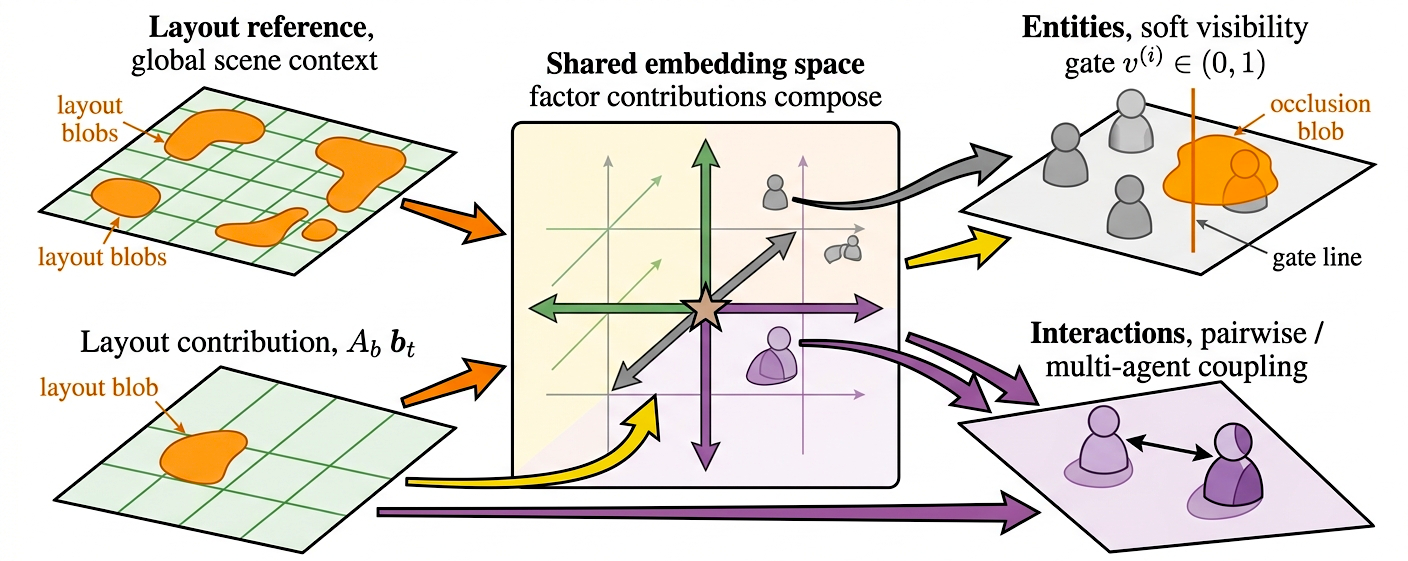
\includegraphics[width=\linewidth]{figures/factor_visual.png}
        \captionof{figure}{
\textbf{\emph{Factorized predictive channels.}}
Context is decomposed into \textbf{\emph{layout}}, visibility-gated
\textbf{\emph{agent}}, and sparse \textbf{\emph{interaction}} coordinates,
then composed in the future JEPA embedding. Separate subspaces preserve spatial
structure, partially observed agents, and multi-agent coupling while limiting
cross-factor leakage.
}
        \label{fig:factorjepa_visual}
    \end{minipage}
    \hfill
    \begin{minipage}[t]{0.48\textwidth}
        \centering
        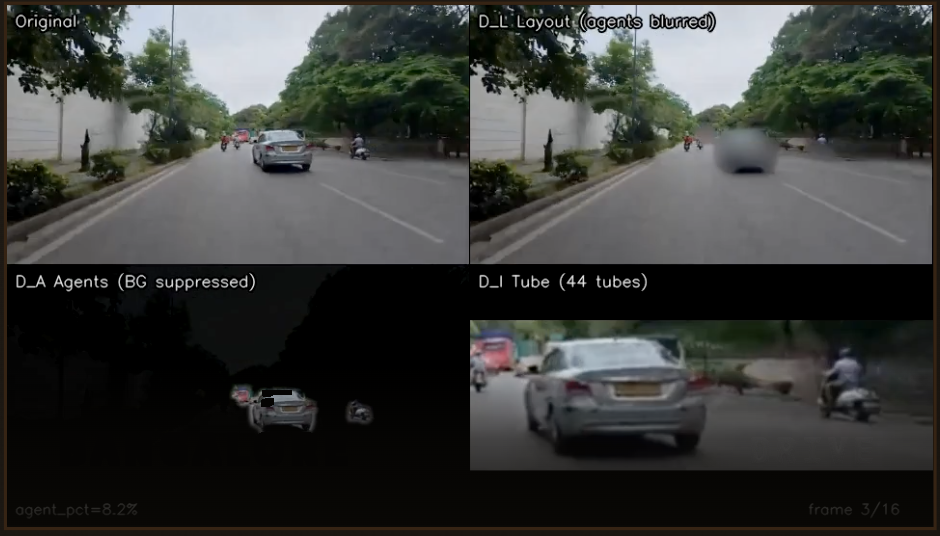
\includegraphics[width=0.85\linewidth]{figures/segmented_scene.png}
        \captionof{figure}{
        \textbf{\emph{DINO-based automatic factor-target construction.}}
        From each input clip, the pipeline derives complementary supervision
        for \textbf{\emph{layout}} $D_L$ by suppressing foreground agents,
        \textbf{\emph{agents}} $D_A$ by suppressing background context, and
        \textbf{\emph{interactions}} $D_I$ through temporally associated agent
        tubes. These targets semantically anchor FactorJEPA's predictive
        channels.
        }
        \label{fig:dino_factor_targets}
    \end{minipage}

    \vspace{-0.5em}
\end{figure*}
\end{comment}


% Preamble
%\usepackage{graphicx}
%\usepackage{caption}

% ---------------------------------------------------------
\begin{figure*}[t]
    \centering

    % -------------------- Agents -------------------- %
    \begin{minipage}[t]{0.325\textwidth}
        \centering
        
\includegraphics[
            width=\linewidth,
            height=0.225\textheight,
            keepaspectratio
        ]{figures/agents_scene.png}
        %\vspace{0.5mm}

        {\small\textbf{(a) Agents}}
    \end{minipage}
    \hfill
    % -------------------- Layout -------------------- %
    \begin{minipage}[t]{0.325\textwidth}
        \centering
        
\includegraphics[
            width=\linewidth,
            height=0.225\textheight,
            keepaspectratio
        ]{figures/layout_scene.png}
        %\vspace{0.5mm}

        {\small\textbf{(b) Layout}}
    \end{minipage}
    \hfill
    % -------------------- Interactions -------------------- %
    \begin{minipage}[t]{0.325\textwidth}
        \centering
        
\includegraphics[
            width=\linewidth,
            height=0.225\textheight,
            keepaspectratio
        ]{figures/interaction_scene.png}
        %\vspace{0.5mm}

        {\small\textbf{(c) Interactions}}
    \end{minipage}

    \vspace{-1em}

    \caption{
\textbf{Factorized decomposition of the same urban scene.}
\textbf{(a)} Agents are isolated from scene context.
\textbf{(b)} Layout highlights persistent spatial structure while retaining
suppressed agent silhouettes.
\textbf{(c)} Interactions show tracklets, residual motion, and sparse pairwise
coupling; arrow direction and length encode motion direction and magnitude,
while solid and dashed edges denote stronger and weaker interactions.
}
    \label{fig:factor_scene_decomposition}
\end{figure*}

\section{\textbf{\emph{FactorJEPA}: Explicitly Factorized Predictive Channels}}
\label{sec:factorjepa}

\paragraph{\textbf{\emph{Motivation.}}}
Let $x$ be a video clip, $M_c$ and $M_t$ its context and target masks,
$f_\theta$ the online encoder, and $\bar f_{\bar\theta}$ the momentum target
encoder. The context representation and stop-gradient future target are

\begin{equation*}
\resizebox{0.98\columnwidth}{!}{$\displaystyle
h_t=f_\theta(M_c\odot x),
\qquad
Y_{t+\Delta}^{\star}
=
\operatorname{sg}\!\left(
\Pi_{M_t}[\bar f_{\bar\theta}(x)]
\right)
\in\mathbb{R}^{m\times d}
$}
\end{equation*}

where $\Pi_{M_t}$ denotes the executed target-selection operator, $m$ the
number of target representations, and $d$ their embedding dimension. A
conventional JEPA predictor learns

\begin{equation*}
g_\phi:(h_t,M_t)
\longmapsto
\widehat{Y}_{t+\Delta}
\in\mathbb{R}^{m\times d}
\end{equation*}

by matching $\widehat{Y}_{t+\Delta}$ to $Y_{t+\Delta}^{\star}$. The objective
specifies \emph{what} to predict, but leaves \emph{how predictive information
is internally organized} unconstrained.

This ambiguity is consequential in \textbf{DENSEWORLD}, where layout, agent
density, visibility, and interaction pressure are strongly correlated. A
high-capacity predictor can exploit \textbf{\emph{shortcut mixtures}}---crowd
texture as a proxy for interaction, visible appearance for object persistence,
or road geometry for motion---without recovering the structure governing scene
evolution.

\textbf{\emph{FactorJEPA}} resolves this ambiguity by replacing the monolithic
predictor with explicit \textbf{\emph{layout}}, \textbf{\emph{agent}}, and
\textbf{\emph{interaction}} channels. A \textbf{\emph{soft visibility gate}}
attenuates uncertain observations, while block-structured regularization limits
\textbf{\emph{cross-factor leakage}}. Together, these components factorize the
future JEPA embedding into semantically anchored coordinates and
factor-specific predictive subspaces.














\subsection{\textbf{\emph{DINOv2-Based Segmentations Agent-Layout-Interactions}}}
\label{sec:factor_target_construction}

For each privacy-filtered clip $x_n$, a frozen DINOv2 pipeline
\cite{oquab2024dinov2} extracts region masks, boxes, descriptors, and
confidences, which are temporally associated into tracklets:
\[
\mathcal P_n
=
\mathcal D_{\mathrm{pre}}
\!\left(\mathcal F_{\mathrm{DINOv2}}(x_n)\right),
\qquad
\mathcal T_n=\mathcal A(\mathcal P_n).
\]
A deterministic structural map converts region geometry, visibility, temporal
continuity, and relative motion into layout, agent, visibility, and interaction
targets with reliability weights:
\[
\Psi_{\mathrm{struct}}(\mathcal P_n,\mathcal T_n)
\longmapsto
\left\{(T_{n,k},q_{n,k})\right\}_{k\in\{L,A,V,I\}} .
\]
Factor-specific heads $\widehat T_{n,k}=P_k(Z_{n,k})$ are trained using
\[
\mathcal L_{\mathrm{factor}}
=
\sum_{k\in\{L,A,I\}}
\frac{
\sum_{n=1}^{N} q_{n,k}\,
\ell_k(\widehat T_{n,k},T_{n,k})
}{
\epsilon+\sum_{n=1}^{N}q_{n,k}
},
\]
while visibility is optimized separately through $\mathcal L_v$.

DINOv2-derived targets supervise training only and are never reused as
evaluation labels. Checkpoints, association and interaction rules, thresholds,
target coverage, and reliability audits are provided in
Appendix~\ref{app:annotation_protocol}.








\begin{figure*}[t]
    \centering

    \begin{minipage}[t]{0.48\textwidth}
        \centering
        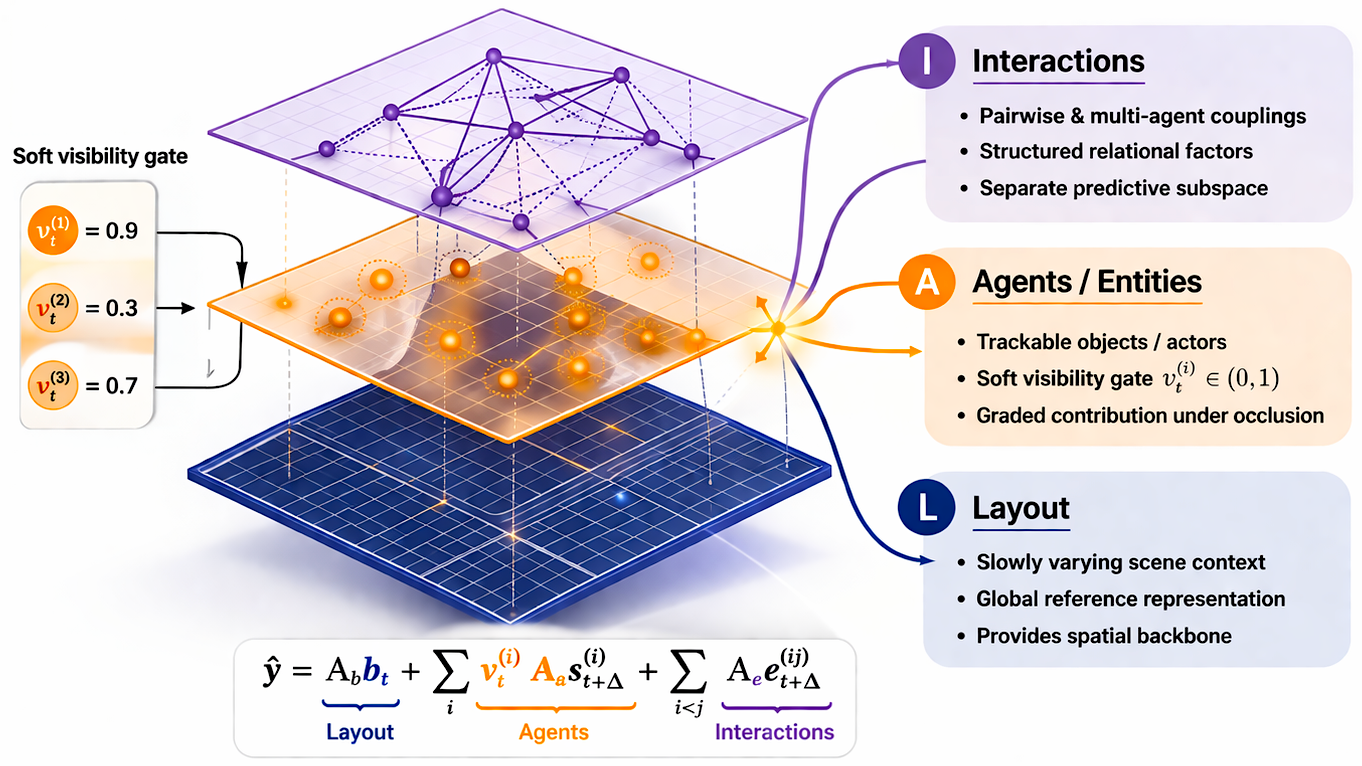
\includegraphics[width=\linewidth]{figures/factors.png}
        \vspace{-1.5em}
        \captionof{figure}{
        \textbf{\emph{Factorized prediction.}}
        \textbf{\emph{FactorJEPA}} composes the target embedding from
        \textbf{\emph{layout}}, \textbf{\emph{agents}}, and
        \textbf{\emph{interactions}}, with a soft visibility gate applied only to
        entity terms.
        }
        \label{fig:factorjepa_factors}
    \end{minipage}
    \hfill
    \begin{minipage}[t]{0.48\textwidth}
        \centering
        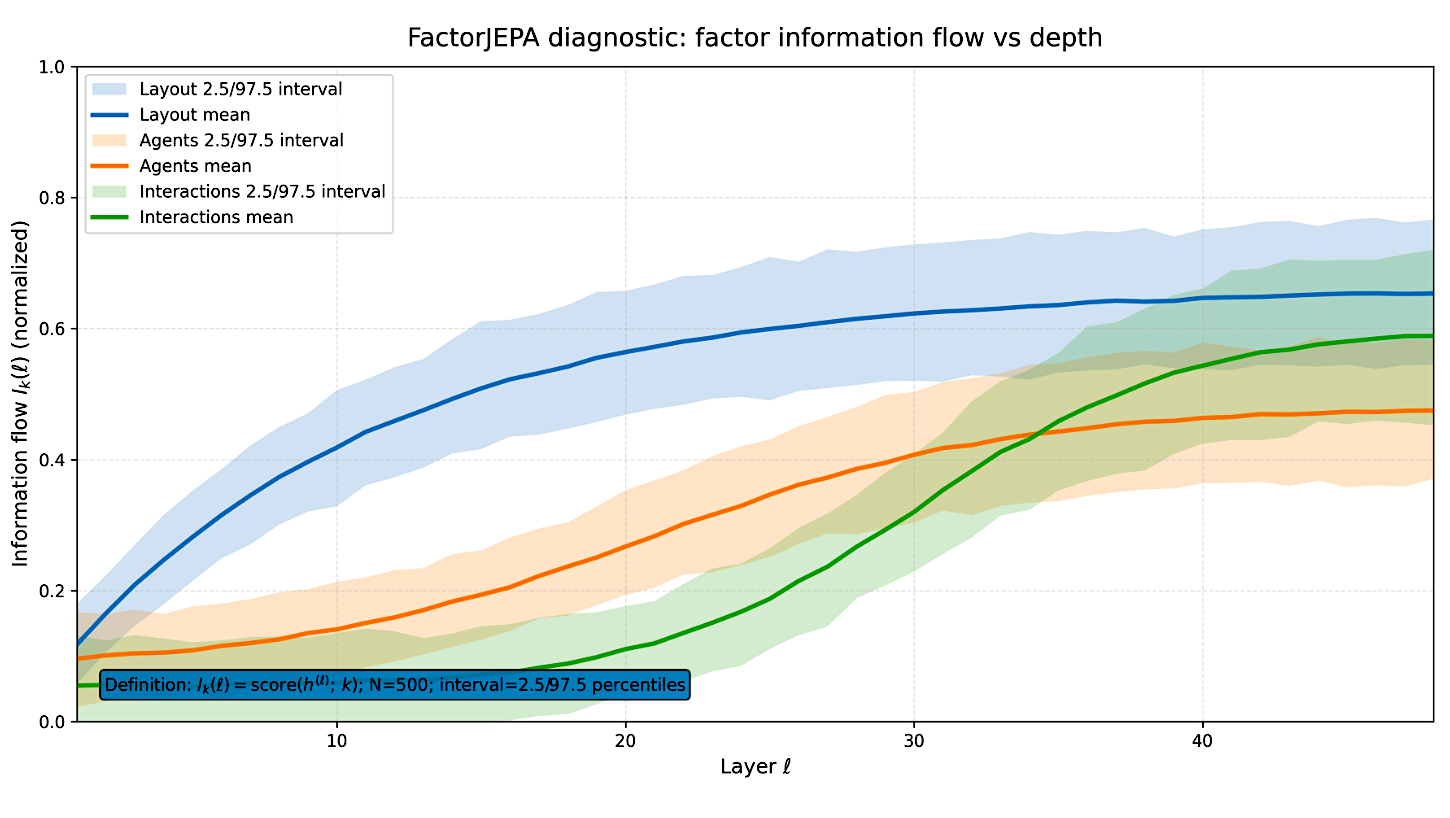
\includegraphics[width=\linewidth]{figures/factor_channels_depth.png}
        \vspace{-1.5em}
        \captionof{figure}{
        \textbf{\emph{Depth-wise factor realization.}}
        Lightweight probes show a staged profile: \textbf{\emph{layout}}
        emerges early, \textbf{\emph{agents}} grow gradually, and
        \textbf{\emph{interactions}} peak in deeper layers.
        }
        \label{fig:factorjepa_channels}
    \end{minipage}

    \vspace{-0.8em}
\end{figure*}










\subsection{\textbf{\emph{Structured Factor Coordinates}}}

For target token $p$, FactorJEPA forms the conditioned query
\[
q_{n,p}=Q\!\left(f_\theta(M_c\odot x_n),\pi_p,M_t\right)
\]
and predicts
\[
c_{n,p}
=
\operatorname{col}
\!\left(c_{n,L,p},c_{n,A,p},c_{n,I,p}\right)
\in\mathbb R^{r_L+r_A+r_I}.
\]
We suppress $p$ below and write $h_n=q_{n,p}$.

\paragraph{\textbf{\emph{Layout.}}}
Slowly varying spatial support is encoded as
\[
c_{n,L}=g_L(h_n),
\qquad
\widehat T_{n,L}=P_L(c_{n,L}).
\]

\paragraph{\textbf{\emph{Visibility-gated agents.}}}
For agent representation $o_n^{(i)}$,
\[
s_n^{(i)}=g_A(h_n,o_n^{(i)}),
\qquad
v_n^{(i)}=\sigma\!\left(g_V(h_n,o_n^{(i)})\right),
\]
and
\[
c_{n,A}
=
\frac{\sum_i v_n^{(i)}s_n^{(i)}}
{\epsilon+\sum_i v_n^{(i)}}.
\]
The gate softly suppresses uncertain or occluded agents without removing them.
Given visibility targets $T_{n,V}^{(i)}$ and reliabilities $q_{n,V}^{(i)}$,
\[
\mathcal L_v
=
-
\frac{
\sum_{n,i}q_{n,V}^{(i)}
\left[
T_{n,V}^{(i)}\log v_n^{(i)}
+
(1-T_{n,V}^{(i)})\log(1-v_n^{(i)})
\right]
}{
\epsilon+\sum_{n,i}q_{n,V}^{(i)}
}.
\]

\paragraph{\textbf{\emph{Sparse interactions.}}}
For each candidate pair $(i,j)\in\mathcal E_n$,
\[
e_n^{(ij)}
=
g_I(h_n,o_n^{(i)},o_n^{(j)}),
\qquad
\bar e_n^{(ij)}
=
\frac{e_n^{(ij)}}{\epsilon+\|e_n^{(ij)}\|_2},
\]
with soft interaction strength
\[
w_n^{(ij)}
=
\sigma\!\left(g_W(h_n,o_n^{(i)},o_n^{(j)})\right).
\]
Let $M_n=\max\{1,|\mathcal E_n|\}$. Then
\[
c_{n,I}
=
\frac{1}{M_n}
\sum_{(i,j)\in\mathcal E_n}
w_n^{(ij)}\bar e_n^{(ij)},
\qquad
c_{n,I}=0
\ \text{if}\ 
\mathcal E_n=\varnothing,
\]
and localized interactions are encouraged through
\[
\mathcal L_{\mathrm{sparse}}
=
\frac{1}{N}
\sum_{n=1}^{N}
\frac{1}{M_n}
\sum_{(i,j)\in\mathcal E_n}
w_n^{(ij)}.
\]
The fixed normalization prevents trivial rescaling of interaction weights and
states.















\subsection{\textbf{\emph{Block-Structured Matrix Factorization}}}

For each factor $k\in\{L,A,I\}$, we stack all target-token coordinates across
the minibatch:
\[
C_k
=
\begin{bmatrix}
(c_{1,k,1})^\top\\[-1mm]
\vdots\\
(c_{1,k,m})^\top\\
\vdots\\
(c_{N,k,m})^\top
\end{bmatrix}
\in\mathbb{R}^{Nm\times r_k}.
\]
The factor coordinates and learned synthesis dictionaries are concatenated as
\[
C=
\begin{bmatrix}
C_L & C_A & C_I
\end{bmatrix},
\qquad
A=
\begin{bmatrix}
A_L & A_A & A_I
\end{bmatrix},
\qquad
A_k\in\mathbb{R}^{d\times r_k}.
\]

FactorJEPA predicts the complete token-level target matrix through
\[
\boxed{
\widehat Y
=
\underbrace{
\begin{bmatrix}
C_L & C_A & C_I
\end{bmatrix}
}_{\text{factor coordinates}}
\underbrace{
\begin{bmatrix}
A_L & A_A & A_I
\end{bmatrix}^{\!\top}
}_{\text{synthesis dictionaries}}
=
CA^\top
}
\]
or, equivalently,
\[
\widehat Y
=
\underbrace{C_LA_L^\top}_{Y_L}
+
\underbrace{C_AA_A^\top}_{Y_A}
+
\underbrace{C_IA_I^\top}_{Y_I}.
\]
Distinct pathways, factor supervision, and dictionaries make the decomposition
architectural rather than post hoc.

For stacked future targets
\[
Y^\star
=
\operatorname{col}
\left(
Y_{1,t+\Delta}^\star,\ldots,Y_{N,t+\Delta}^\star
\right)
\in\mathbb{R}^{Nm\times d},
\]
the JEPA objective is
\[
\mathcal L_{\mathrm{JEPA}}
=
\frac{1}{Nm}
\left\|
\widehat Y-Y^\star
\right\|_F^2.
\]
The corresponding $m$ rows are unstacked per clip, preserving the complete
future-token geometry.















\begin{figure*}[ht!]
    \centering

    %-------------------- Left figure --------------------%
    \begin{minipage}[t]{0.485\textwidth}
        \vspace{0pt}
        \centering
        
\includegraphics[
            width=\linewidth
        ]{figures/forest_plot_best_ci_paper.pdf}

        \vspace{-0.5em}
        \captionof{figure}{
\textbf{\emph{FactorJEPA vs. the strongest competitor across scale
and data regimes.}}
Bars report FactorJEPA's advantage in units of the paired-difference
95\% confidence interval; the dashed line marks statistical separation at
$1\times$. Under matched stratified 10k protocol, FactorJEPA separates on
Future-frame L1 and Causal L1 at both scales, and on Mask-ratio slope at 1B,
while trailing on Motion cosine---revealing a consistent prediction--motion
trade-off. With full 115k-clip training at 1B, it separates strongly on all
four primary diagnostics, reaching $43.3\times$ for Mask-ratio slope,
$33.2\times$ for Future-frame L1, $20.0\times$ for Motion cosine, and
$13.9\times$ for Causal L1.
}
        \label{fig:frozen_forest}
    \end{minipage}
    \hfill
    %-------------------- Right figure --------------------%
    \begin{minipage}[t]{0.485\textwidth}
        \vspace{0pt}
        \centering
        
\includegraphics[
            width=\linewidth
        ]{figures/eval_scorecard_winbars.pdf}

        \vspace{-0.5em}
        \captionof{figure}{
\textbf{\emph{Evaluation scorecard across 2B and 1B scales.}}
Frozen, conventionally adapted, parameter-efficient, and factorized
V-JEPA~2.1 variants are compared across predictive, motion, semantic,
and temporal diagnostics. Bars report performance with 95\% BCa
intervals where available.
}
        \label{fig:eval_scorecard}
    \end{minipage}

    \vspace{-1.2em}
\end{figure*}









\subsection{\textbf{\emph{Semantic Anchoring and Channel Separation}}}

The factorization $\widehat Y=CA^\top$ is non-unique: for any invertible
$R$,
\[
CA^\top=(CR)(AR^{-\top})^\top.
\]
Thus, the JEPA objective alone permits rotations and cross-block mixing.
Factor-specific heads
\[
\widehat T_k=C_kP_k^\top,
\qquad k\in\{L,A,I\},
\]
together with $\mathcal L_{\mathrm{factor}}$, anchor the blocks to layout,
agents, and interactions. FactorJEPA therefore claims semantic block
separation, not coordinate-level identifiability.

To suppress residual cross-channel shortcuts, let
$\Gamma_{kk'}$ denote the empirical covariance between channel outputs
$Y_k$ and $Y_{k'}$. We penalize linear and nonlinear leakage through
\[
\mathcal L_{\mathrm{sep}}
=
\underbrace{
2\sum_{k<k'}\|\Gamma_{kk'}\|_F^2
}_{\mathcal L_{\mathrm{cov}}}
+
\beta_{\mathrm{nlin}}
\underbrace{
\sum_{k<k'}
\frac{
\operatorname{tr}(\bar K_k\bar K_{k'})
}{
\|\bar K_k\|_F\|\bar K_{k'}\|_F+\epsilon
}
}_{\mathcal L_{\mathrm{nlin}}},
\]
where $\bar K_k$ is the centered RBF Gram matrix for channel $k$.
This suppresses cross-channel dependence while leaving within-channel
variation unconstrained; it does not imply statistical or causal
independence.

\paragraph{\textbf{\emph{Leakage diagnostic.}}}
We freeze FactorJEPA and train fixed-capacity probes from channel $Y_k$ to
factor target $T_{k'}$. With held-out probe score $S_{k\rightarrow k'}$ and
constant-predictor score $S_{0\rightarrow k'}$, normalized leakage is
\[
\operatorname{Leak}(k\!\rightarrow\!k')
=
\frac{
S_{k\rightarrow k'}-S_{0\rightarrow k'}
}{
S_{k'\rightarrow k'}-S_{0\rightarrow k'}+\epsilon
},
\qquad k\neq k'.
\]
Effective separation requires strong diagonal predictability and low
off-diagonal leakage. Full definitions and probe protocols are provided in
Appendix~\ref{app:factor_separation}.






\begin{comment}
    

\begin{figure*}[ht!]
    \centering
    
\includegraphics[width=0.8\textwidth]
    {figures/eval_scorecard_winbars.pdf}
    \caption{
    \textbf{\emph{Complete evaluation scorecard at 2B and 1B scales.}}
    We compare frozen, conventionally adapted, parameter-efficient, and
    factorized V-JEPA~2.1 variants across 15 semantic, predictive, motion, and
    temporal-coherence diagnostics. Bars report test performance with 95\% BCa
    confidence intervals where available. The four headline diagnostics are
    Future-frame L1, Causal L1, Motion cosine, and Mask-ratio slope.
    }
    \label{fig:eval_scorecard}
    \vspace{-0.6em}
\end{figure*}
\end{comment}



\begin{figure}[t]
    \centering
    
\includegraphics[width=0.65\columnwidth]
    {figures/scale_replication_single.pdf}
    \caption{
    \textbf{\emph{Causal future-block rankings replicate across model scales.}}
    Each point represents one adaptation method, comparing its causal
    future-block L1 score with the ViT-G 2B backbone on the horizontal axis
    and the ViT-g 1B backbone on the vertical axis; lower values are better.
    FactorJEPA variants are shown in green, and the dashed line denotes
    equal scores across scales. The strong Spearman correlation
    ($\rho=0.979$) shows that the relative method ordering is highly
    preserved when scaling from 2B to 1B.
    }
    \label{fig:scale_replication}
    \vspace{-0.6em}
\end{figure}



\subsection{\textbf{\emph{Predictor Surgery}}}

FactorJEPA is initialized from a pretrained V-JEPA model. The online encoder,
momentum target encoder, target construction, and masking policy are retained.
Only the monolithic predictor is replaced:

\begin{equation*}
\Theta_{\mathrm{pred}}
\longrightarrow
\Theta_{\mathrm{fact}}
=
\left\{
\Theta_L,\Theta_A,\Theta_I,\Theta_V,\Theta_W,A
\right\}.
\end{equation*}

Training is restricted to the factorized predictor and the top $K$ encoder
blocks:

\begin{equation*}
\Theta_{\mathrm{train}}
=
\Theta_{\mathrm{fact}}
\cup
\Theta_{\mathrm{top}\text{-}K}.
\end{equation*}

The lower encoder blocks and momentum target network follow the frozen or
momentum-updated protocol of the underlying V-JEPA implementation.

The final objective is
\begin{equation*}
\boxed{
\begin{aligned}
\mathcal L
&=
\mathcal L_{\mathrm{JEPA}}
+
\lambda_{\mathrm{sep}}\mathcal L_{\mathrm{sep}}
+
\lambda_{\mathrm{sparse}}\mathcal L_{\mathrm{sparse}}\\
&\quad+
\lambda_v\mathcal L_v
+
\lambda_{\mathrm{sup}}\mathcal L_{\mathrm{factor}}.
\end{aligned}
}
\end{equation*}

Each term has a distinct role:
\begin{equation*}
\begin{array}{rcl}
\mathcal L_{\mathrm{JEPA}}
&:&
\text{future-latent prediction},\\
\mathcal L_{\mathrm{sep}}
&:&
\text{cross-channel leakage suppression},\\
\mathcal L_{\mathrm{sparse}}
&:&
\text{interaction locality},\\
\mathcal L_v
&:&
\text{visibility calibration},\\
\mathcal L_{\mathrm{factor}}
&:&
\text{semantic anchoring}.
\end{array}
\end{equation*}






\subsection{\textbf{\emph{Depth-Wise Factor Realization}}}
\label{sec:depth_analysis}

Although the factorization acts at the predictor, we test how factor information
becomes linearly accessible across encoder depth. Let

\begin{equation*}
H^{(\ell)}
=
\begin{bmatrix}
h_1^{(\ell)}&\cdots&h_N^{(\ell)}
\end{bmatrix}^{\!\top}
\in\mathbb{R}^{N\times d_\ell}
\end{equation*}

denote the representations at layer $\ell$. For each factor
$k\in\{L,A,I\}$, we fit a regularized linear probe on the training split:

\begin{equation*}
\resizebox{0.98\columnwidth}{!}{$\displaystyle
W_k^{(\ell)}
=
\arg\min_W
\left\|
H_{\mathrm{train}}^{(\ell)}W-T_{k,\mathrm{train}}
\right\|_F^2
+
\lambda_{\mathrm{probe}}\|W\|_F^2
$}
\end{equation*}

The held-out depth-wise factor score is

\begin{equation*}
I_k(\ell)
=
\operatorname{score}_k
\left(
H_{\mathrm{test}}^{(\ell)}W_k^{(\ell)},
T_{k,\mathrm{test}}
\right).
\end{equation*}

Distinct onset and growth profiles indicate that layout, agent, and interaction
information becomes accessible at different depths. This is a representation
diagnostic, not a neuron-level or causal decomposition.















































\section{\textbf{Experiments \& Evaluation}}
\label{sec:experiments}

We ask whether FactorJEPA improves V-JEPA's \emph{predictive structure}, rather
than only its downstream semantics or linear accessibility. We evaluate four
complementary diagnostics: \textbf{Future-frame L1}, \textbf{Causal L1},
\textbf{Mask-ratio slope}, and \textbf{Motion cosine}. Together, they probe
future-latent fidelity, intervention sensitivity, robustness under partial
observability, and accessible motion information, distinguishing improved
forecasting from semantic alignment or easier linear readout alone.

\subsection{\textbf{\emph{Evaluator Independence and Audit Split}}}
\label{sec:evaluator_independence}

To prevent agreement with the pseudo-label generator from being mistaken for
improved world modeling, we strictly separate training-target construction from
evaluation. DINOv2-derived targets are constructed only on the training split:
\begin{equation*}
\mathcal T_{\mathrm{train}}
=
\Psi_{\mathrm{struct}}
\left(
\mathcal F_{\mathrm{DINOv2}}(x)
\right),
\qquad
x\in\mathcal D_{\mathrm{train}}.
\end{equation*}

Primary factor-specific evaluation uses a city-disjoint audit split
$\mathcal D_{\mathrm{audit}}$, whose agent masks, visibility states,
interaction pairs, and intervention regions are independently annotated:
\begin{equation*}
\mathcal D_{\mathrm{train}}
\cap
\mathcal D_{\mathrm{audit}}
=
\varnothing,
\qquad
\mathcal T_{\mathrm{audit}}
=
\Psi_{\mathrm{human}}(x).
\end{equation*}

Audit annotations are excluded from training, model selection, threshold
selection, and hyperparameter tuning. City disjointness further limits
scene-specific or geographic memorization. Future-frame L1 and Mask-ratio slope
use the frozen V-JEPA target encoder; Motion cosine uses an independently
frozen motion estimator; and RGB Agent F1 uses an external detector supplying
neither FactorJEPA supervision nor DINOv2 preprocessing. Thus, no headline
evaluator reuses FactorJEPA's pseudo-label generator or training targets.

\subsection{\textbf{\emph{Protocol and Comparisons}}}

We evaluate V-JEPA~2.1 at two scales: ViT-G with approximately 2B parameters
and ViT-g with approximately 1B parameters. Both are evaluated under a matched
stratified 10k-clip regime; ViT-g is additionally trained on the full
115k-clip corpus. Full-scale ViT-G training is omitted under the declared
compute budget because it requires approximately twice the 1B cost.

Comparisons span the frozen backbone, full and parameter-efficient fine-tuning,
continual SSL, LP-FT, LoRA, DoRA, Auto-RGN, WiSE-FT,
\textbf{FactorJEPA-RAW}, and full \textbf{FactorJEPA}. FactorJEPA-RAW retains
the factorized predictor but removes factor-target supervision, yielding
\begin{equation*}
\resizebox{0.98\columnwidth}{!}{$\displaystyle
\underbrace{\{\text{LoRA},\text{DoRA},\text{Auto-RGN}\}}_{\text{generic adaptation}}
\;\longrightarrow\;
\underbrace{\text{FactorJEPA-RAW}}_{\text{factorized architecture}}
\;\longrightarrow\;
\underbrace{\text{FactorJEPA}}_{\text{architecture + factor curriculum}}
$}
\end{equation*}
This attribution chain separates gains from generic adaptation, predictor
factorization, and structured supervision. The experiments therefore test
whether explicit \textbf{layout--agent--interaction structure} improves future
prediction beyond a matched monolithic JEPA predictor.

Within each regime, all methods use identical clips, masking policies,
optimization steps, evaluation splits, and metric implementations. We report
per-encoder test results with paired 95\% BCa bootstrap confidence intervals.

\subsection{\textbf{\emph{Four Diagnostics of Predictive Structure}}}

\paragraph{\textbf{\emph{Future-frame L1 ($\downarrow$).}}}
Normalized L1 distance between predicted and target future embeddings; lower
values indicate \textbf{\emph{more accurate future-latent prediction}}.

\paragraph{\textbf{\emph{Causal L1 ($\downarrow$).}}}
For each independently annotated intervention region $a$, we apply the same
controlled edit $\mathcal I_a$ and compare its effect on predicted and target
future latents:
\begin{equation*}
\resizebox{0.98\columnwidth}{!}{$\displaystyle
\widehat\Delta_a
=
\widehat Y\!\left(\mathcal I_a(x)\right)-\widehat Y(x),
\qquad
\Delta_a^\star
=
\operatorname{sg}\!\left[
\bar f_{\bar\theta}\!\left(\mathcal I_a(x)\right)
-
\bar f_{\bar\theta}(x)
\right].
$}
\end{equation*}
\begin{equation*}
\operatorname{CausalL1}
=
\frac{1}{|\mathcal A|}
\sum_{a\in\mathcal A}
\frac{
\|\widehat\Delta_a-\Delta_a^\star\|_1
}{
\epsilon+\|\Delta_a^\star\|_1
}.
\end{equation*}
Intervention regions and types come from independent audit annotations, not
DINOv2 predictions. The metric evaluates consistency with
intervention-induced changes, not causal identification.

\paragraph{\textbf{\emph{Mask-ratio slope ($\downarrow$).}}}
Increase in prediction error as visual evidence is progressively masked; a
smaller slope indicates \textbf{\emph{greater robustness under partial
observability}}.

\paragraph{\textbf{\emph{Motion cosine ($\uparrow$).}}}
Cosine alignment between linearly decoded and target motion descriptors; higher
values indicate \textbf{\emph{more linearly accessible motion information}}.

Together, these diagnostics distinguish improved future modeling from gains
limited to semantic decoding, a single masking level, or convenient linear
representation.

\subsection{\textbf{\emph{Performance Across Scale and Data Regimes}}}

Figures~\ref{fig:frozen_forest} and~\ref{fig:eval_scorecard} summarize the
primary evidence. Under the matched stratified 10k protocol, FactorJEPA
separates from the strongest competitor on Future-frame L1
($6.3\times$/$4.8\times$ CI widths) and Causal L1
($2.3\times$/$2.7\times$) at 2B/1B. Mask-ratio slope remains within the
confidence interval at 2B ($0.9\times$) but separates at 1B
($1.9\times$). Motion cosine instead favors generic fine-tuning
($-14.5\times$/$-9.2\times$), exposing a limited-data
prediction--motion trade-off.

Full 115k-clip training changes this profile decisively. At 1B, FactorJEPA
separates on all four primary diagnostics, reaching
\textbf{\emph{$43.3\times$}} for Mask-ratio slope,
\textbf{\emph{$33.2\times$}} for Future-frame L1,
\textbf{\emph{$20.0\times$}} for Motion cosine, and
\textbf{\emph{$13.9\times$}} for Causal L1
(Figure~\ref{fig:frozen_forest}). These values denote separation in paired
confidence-interval units, not multiplicative performance gains.

Figure~\ref{fig:eval_scorecard} further shows that the gains are
\textbf{\emph{structured rather than universal}}. FactorJEPA leads on
predictive fidelity, intervention sensitivity, and robustness-oriented
diagnostics, while generic adaptation remains competitive on several
frame-timing and temporal-coherence measures. The improvement therefore targets
the information required to forecast crowded, partially observed scenes rather
than uniformly shifting unrelated metrics.

\subsection{\textbf{\emph{Prediction--Motion Trade-off}}}

Under stratified 10k training, FactorJEPA improves future prediction,
intervention consistency, and masking robustness while conceding maximally
linear motion readout to conventional fine-tuning. This suggests that, with
limited data, the factorized objective prioritizes motion information useful
for structured forecasting rather than motion that is easiest to recover
linearly.

Crucially, full 115k training reverses this deficit: Motion cosine becomes a
strongly separated win while the predictive gains increase further. The
trade-off is therefore \textbf{\emph{data- and optimization-dependent}}, not an
intrinsic limitation of layout--agent--interaction factorization. With
sufficient interaction coverage, FactorJEPA preserves both structured
prediction and accessible motion.

\subsection{\textbf{\emph{Cross-Scale Replication}}}

We test whether adaptation rankings survive the transition from the 2B backbone
to the approximately half-cost 1B backbone. For diagnostic $k$,
\begin{equation*}
\rho_k
=
\operatorname{Spearman}
\left(
\mathbf s_k^{2\mathrm B},
\mathbf s_k^{1\mathrm B}
\right),
\end{equation*}
where $\mathbf s_k^{2\mathrm B}$ and $\mathbf s_k^{1\mathrm B}$ contain
per-method scores at the two scales.

As Figure~\ref{fig:scale_replication} illustrates, Causal L1 yields
$\rho=0.979$, Motion cosine $\rho=0.952$, Future-frame L1
$\rho=0.938$, and Mask-ratio slope $\rho=0.895$. These are the four strongest
cross-scale correlations. Twelve of fifteen diagnostics retain broadly
consistent rankings, while Temporal-order, Teacher-free gap, and Rollout drift
do not transfer reliably.

The result shows that the relative behavior of adaptation strategies is largely
backbone-invariant. Both FactorJEPA's predictive gains and its limited-data
motion trade-off reflect stable method ordering rather than artifacts of one
model size. The high correlations also establish the 1B backbone as a faithful
lower-cost proxy for screening adaptation choices before full-scale 2B
training.













































\begin{comment}
    
\section{\textbf{From Future Latents to Visible Futures}}
\label{sec:latent_to_rgb}

JEPA models predict in embedding space, making their forecasts difficult to
inspect directly. We therefore introduce a \textbf{\emph{Cosmos-initialized
latent-to-RGB decoder}} that renders FactorJEPA's predicted future embedding as
an RGB frame. The decoder does not perform forecasting or alter FactorJEPA; it
provides a visual interface to the future already predicted in latent space.

\subsection{\textbf{\emph{Latent Transport and RGB Decoding}}}

FactorJEPA produces a future embedding
$\widehat Y_{t+\Delta}\in\mathbb{R}^{m\times d_J}$, whereas the Cosmos decoder
expects a spatial conditioning tensor. We introduce a learned transport
operator

\begin{equation*}
\mathcal T_\omega:
\mathbb{R}^{m\times d_J}
\longrightarrow
\mathbb{R}^{h\times w\times d_C}
\end{equation*}

that aligns the JEPA token geometry, dimensionality, and feature statistics with
the Cosmos decoding space. The rendered future is

\begin{equation*}
\boxed{
\widehat x_{t+\Delta}
=
\mathcal G_{\psi_C}
\left(
\mathcal T_\omega(
\widehat Y_{t+\Delta})
\right)
}
\end{equation*}

where $\mathcal G_{\psi_C}$ is initialized from the corresponding Cosmos
component~\cite{nvidia2025cosmos}. At inference, the decoder receives only
FactorJEPA's predicted future latent; the ground-truth future frame is never
provided.





\begin{figure*}[ht!]
    \centering
    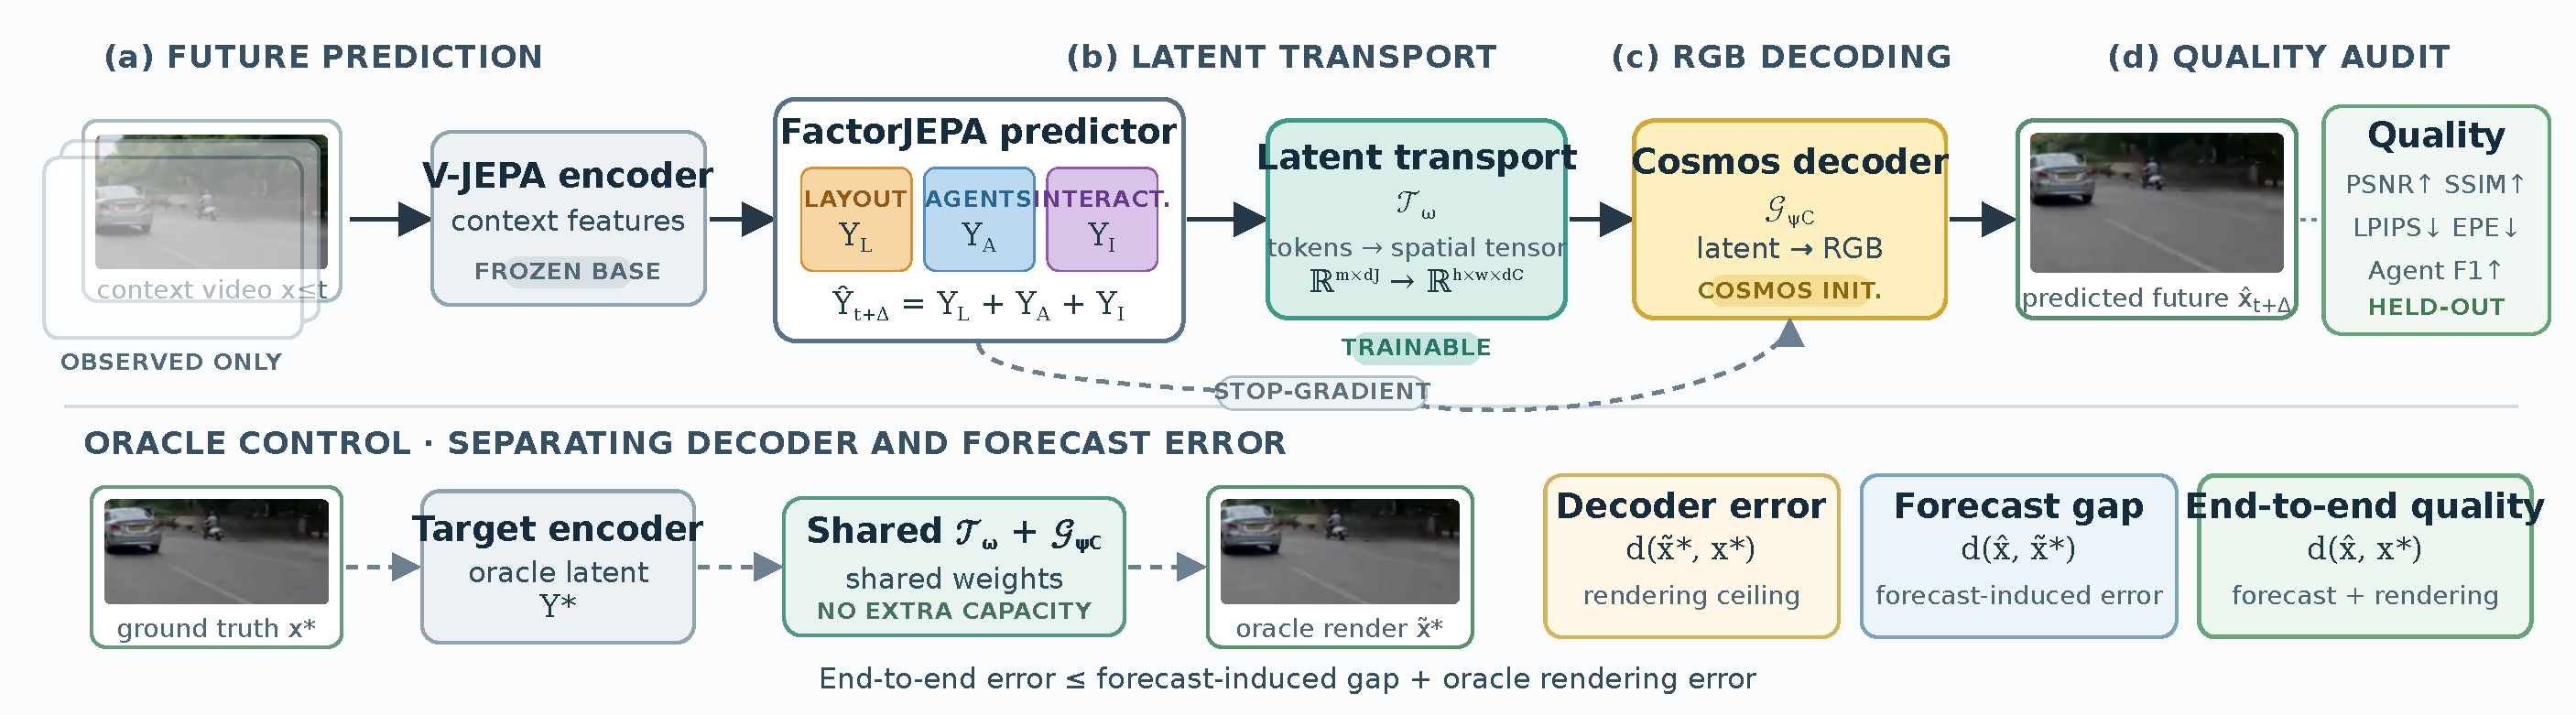
\includegraphics[width=\textwidth]
    {figures/latent_to_rgb_pipeline.pdf}
    \vspace{-0.6em}
    \caption{
    \textbf{\emph{From factorized future latents to visible futures.}}
    FactorJEPA predicts \textbf{\emph{layout}}, \textbf{\emph{agent}}, and
    \textbf{\emph{interaction}} channels, which a learned transport maps into
    the conditioning space of a \textbf{Cosmos-initialized decoder} to render
    the predicted future RGB frame. An oracle reconstruction from the target
    future latent separates \textbf{\emph{decoder error}} from the
    \textbf{\emph{forecast-induced gap}}, while their combination measures
    \textbf{\emph{end-to-end prediction quality}}. RGB reconstruction gradients
    are stopped before FactorJEPA.
    }
    \label{fig:latent_to_rgb_pipeline}
    \vspace{-1.0em}
\end{figure*}

\subsection{\textbf{\emph{Decoder Adaptation}}}

We first train the decoder to invert target-encoder latents. Let
$Y_{t+\Delta}^{\star}$ be the stop-gradient target latent paired with the
observed future frame $x_{t+\Delta}$. Its oracle reconstruction is

\begin{equation*}
\widetilde x_{t+\Delta}^{\star}
=
\mathcal G_{\psi_C}
\left(
\mathcal T_\omega(
Y_{t+\Delta}^{\star})
\right).
\end{equation*}

To reduce the distribution gap between target and predicted latents, the
decoder is additionally exposed to stop-gradient FactorJEPA predictions. The
training objective is

\begin{equation*}
\resizebox{0.98\columnwidth}{!}{$\displaystyle
\boxed{
\mathcal L_{\mathrm{decode}}
=
\mathbb E
\left[
\ell_{\mathrm{RGB}}
\left(
\widetilde x_{t+\Delta}^{\star},
x_{t+\Delta}
\right)
\right]
+
\eta\,
\mathbb E
\left[
\ell_{\mathrm{RGB}}
\left(
\widehat x_{t+\Delta},
x_{t+\Delta}
\right)
\right]
}
$}
\end{equation*}

FactorJEPA is frozen throughout decoder training, and
$\operatorname{sg}(\widehat Y_{t+\Delta})$ is used in the second term. Thus,
RGB reconstruction cannot modify the world model or its latent forecasts.
The executed reconstruction losses, Cosmos checkpoint, transport architecture,
latent normalization, and value of $\eta$ are reported in
Appendix~\ref{app:latent_rgb_details}.

\subsection{\textbf{\emph{Separating Forecast and Decoder Error}}}

A decoded prediction can fail because the future latent is inaccurate or
because the decoder cannot perfectly invert a correct latent. We separate these
sources using the oracle reconstruction:

\begin{equation*}
\begin{aligned}
\left\|
\widehat x_{t+\Delta}-x_{t+\Delta}
\right\|
&\le
\underbrace{
\left\|
\widehat x_{t+\Delta}
-
\widetilde x_{t+\Delta}^{\star}
\right\|
}_{\text{forecast-induced rendering gap}}
\\[-1mm]
&\quad+
\underbrace{
\left\|
\widetilde x_{t+\Delta}^{\star}
-
x_{t+\Delta}
\right\|
}_{\text{oracle decoder error}}.
\end{aligned}
\end{equation*}

The oracle term measures the decoder's reconstruction ceiling; the forecast
term measures the visible effect of replacing the target latent with
FactorJEPA's prediction. This decomposition prevents decoder limitations from
being attributed to the world model.

\subsection{\textbf{\emph{Evaluating RGB Prediction Quality}}}

We evaluate held-out reconstructions along five complementary axes:
\textbf{\emph{(i) pixel fidelity}} using PSNR,
\textbf{\emph{(ii) structural fidelity}} using SSIM,
\textbf{\emph{(iii) perceptual similarity}} using LPIPS,
\textbf{\emph{(iv) motion fidelity}} using optical-flow endpoint error, and
\textbf{\emph{(v) crowded-scene fidelity}} using agent F1 from a frozen,
independent evaluator. No evaluator used for RGB assessment supplies
FactorJEPA's factor targets.

For motion fidelity, let $x_t$ be the final context frame and define

\begin{equation*}
F^\star
=
\operatorname{Flow}(x_t,x_{t+\Delta}),
\qquad
\widehat F
=
\operatorname{Flow}(x_t,\widehat x_{t+\Delta}).
\end{equation*}

We report

\begin{equation*}
\operatorname{EPE}_{\mathrm{flow}}
=
\frac{1}{HW}
\sum_{p}
\left\|
\widehat F(p)-F^\star(p)
\right\|_2,
\end{equation*}

using the same frozen flow estimator for every method. This tests whether the
rendered future moves correctly, rather than only whether it appears realistic.

The evaluation compares four latent sources under the
\textbf{\emph{same decoder}}: target latents provide the oracle ceiling;
standard V-JEPA predictions test monolithic forecasting;
FactorJEPA-RAW isolates architectural factorization; and full FactorJEPA
measures architecture plus factor supervision.

\begin{table}[ht!]
\centering
\caption{
\textbf{Latent-to-RGB prediction on held-out clips.}
Oracle decoding isolates decoder capacity; predicted latents evaluate the
complete world-model--decoder pipeline. All methods share the same
Cosmos-initialized decoder.
}
\label{tab:latent_rgb}
\vspace{-0.4em}
\scriptsize
\setlength{\tabcolsep}{3pt}
\renewcommand{\arraystretch}{1.10}
\resizebox{\columnwidth}{!}{%
\begin{tabular}{lccccc}
\toprule
\textbf{Latent source}
& \shortstack{\textbf{PSNR}\\$\uparrow$}
& \shortstack{\textbf{SSIM}\\$\uparrow$}
& \shortstack{\textbf{LPIPS}\\$\downarrow$}
& \shortstack{\textbf{Flow EPE}\\$\downarrow$}
& \shortstack{\textbf{Agent F1}\\$\uparrow$} \\
\midrule
Target latent (oracle)    & -- & -- & -- & -- & -- \\
V-JEPA                    & -- & -- & -- & -- & -- \\
FactorJEPA-RAW            & -- & -- & -- & -- & -- \\
\textbf{FactorJEPA}       & -- & -- & -- & -- & -- \\
\bottomrule
\end{tabular}%
}
\vspace{-0.7em}
\end{table}

\subsection{\textbf{\emph{Factor-Level Visual Inspection}}}

The factorized prediction also enables controlled pixel-space inspection.
Writing

\begin{equation*}
\widehat Y
=
Y_L+Y_A+Y_I,
\end{equation*}

we decode a factor-removed future

\begin{equation*}
\widehat x^{(-k)}
=
\mathcal G_{\psi_C}
\left(
\mathcal T_\omega(
\widehat Y-Y_k)
\right),
\qquad
k\in\{L,A,I\},
\end{equation*}

and define its influence map as

\begin{equation*}
\Delta_k
=
\left|
\widehat x-\widehat x^{(-k)}
\right|.
\end{equation*}

These maps reveal where each predictive channel changes the rendered future:
layout primarily affects spatial support, agents affect object occupancy and
appearance, and interactions affect localized multi-agent evolution. They are
factor-ablation diagnostics, not causal pixel explanations.

\paragraph{\textbf{\emph{Takeaway.}}}
The Cosmos-initialized decoder turns FactorJEPA from a
\textbf{\emph{silent latent simulator}} into a visually inspectable world
model. Oracle decoding measures what can be reconstructed from a correct latent;
predicted decoding shows what FactorJEPA expects to happen; and factor ablations
expose which structured channel supports each visible change.

\end{comment}











